% Supplementary figures for the revised decomposition section.

\subsection{Additional figures}
\label{app:decomp_figures}
\label{ssec:decomposition_figures}

\begin{figure}[!htbp]
\centering
\IfFileExists{../resources/decomposition/figures/figure_02_binned_scatter_exit_lowed_notitle.pdf}{%
  
\includegraphics[width=0.72\textwidth]{../resources/decomposition/figures/figure_02_binned_scatter_exit_lowed_notitle.pdf}%
}{%
  \fbox{\parbox[c][2in][c]{0.72\textwidth}{\centering Placeholder for municipality-level binned scatter.}}%
}
\caption{Municipality-level exit rate and baseline low-education share}
\label{fig:decomp_scatter_muni}
\label{fig:decomp_scatter_muni_app}

\vspace{0.75em}
\begin{minipage}{\textwidth}
{\footnotesize \textbf{Note:} This figure is a descriptive complement to the main allocation results. Because the dependent variable is itself generated by the cohort framework, the figure should be read as supportive heterogeneity rather than independent identification. \par}
\end{minipage}
\end{figure}

\begin{figure}[!htbp]
\centering
\IfFileExists{../resources/decomposition/figures/figure_03_state_scatter_exit_lowed_notitle.pdf}{%
  
\includegraphics[width=0.72\textwidth]{../resources/decomposition/figures/figure_03_state_scatter_exit_lowed_notitle.pdf}%
}{%
  \fbox{\parbox[c][2in][c]{0.72\textwidth}{\centering Placeholder for state-level scatter.}}%
}
\caption{State-level exit rate and baseline low-education share}
\label{fig:decomp_scatter_state}
\label{fig:decomp_scatter_state_app}

\vspace{0.75em}
\begin{minipage}{\textwidth}
{\footnotesize \textbf{Note:} State aggregation is useful for visual context but too coarse for identification. If retained, the text should emphasize the descriptive regional pattern rather than treat this figure as a test. \par}
\end{minipage}
\end{figure}

\begin{figure}[!htbp]
\centering
\IfFileExists{../resources/decomposition/figures/figure_04_interaction_coefficients_notitle.pdf}{%
  
\includegraphics[width=0.72\textwidth]{../resources/decomposition/figures/figure_04_interaction_coefficients_notitle.pdf}%
}{%
  \fbox{\parbox[c][2in][c]{0.72\textwidth}{\centering Placeholder for interaction coefficient plot.}}%
}
\caption{Supplementary interaction coefficients}
\label{fig:decomp_coefficients}
\label{fig:decomp_coefficients_app}

\vspace{0.75em}
\begin{minipage}{\textwidth}
{\footnotesize \textbf{Note:} This figure should remain in the appendix unless the full pipeline is bootstrapped. Otherwise the reported uncertainty conditions on a generated dependent variable and does not capture first-stage uncertainty from the cohort allocation itself. \par}
\end{minipage}
\end{figure}

\begin{figure}[!htbp]
\centering
\IfFileExists{../resources/decomposition/figures/figure_05_share_by_age_band_notitle.pdf}{%
  
\includegraphics[width=0.72\textwidth]{../resources/decomposition/figures/figure_05_share_by_age_band_notitle.pdf}%
}{%
  \fbox{\parbox[c][2in][c]{0.72\textwidth}{\centering Placeholder for age-profile figure.}}%
}
\caption{Full age profile of exit and record updating}
\label{fig:decomp_age_share}
\label{fig:decomp_age_share_app}

\vspace{0.75em}
\begin{minipage}{\textwidth}
{\footnotesize \textbf{Note:} The main text should draw attention to the working-age concentration of re-labeling rather than to the noisy oldest bins. If a redesigned main-text age figure is later added, it should focus on ages 25--64 or 35--64 and relegate the full profile to this appendix. \par}
\end{minipage}
\end{figure}

\begin{figure}[p]
    \caption{BJS imputation decomposition event studies over the 2006 baseline}
    \label{fig:appendix-decomp-event-components}
    \label{fig:appendix-decomp-event-combined}
    \centering
    \begin{subfigure}[b]{0.49\textwidth}
        \centering
        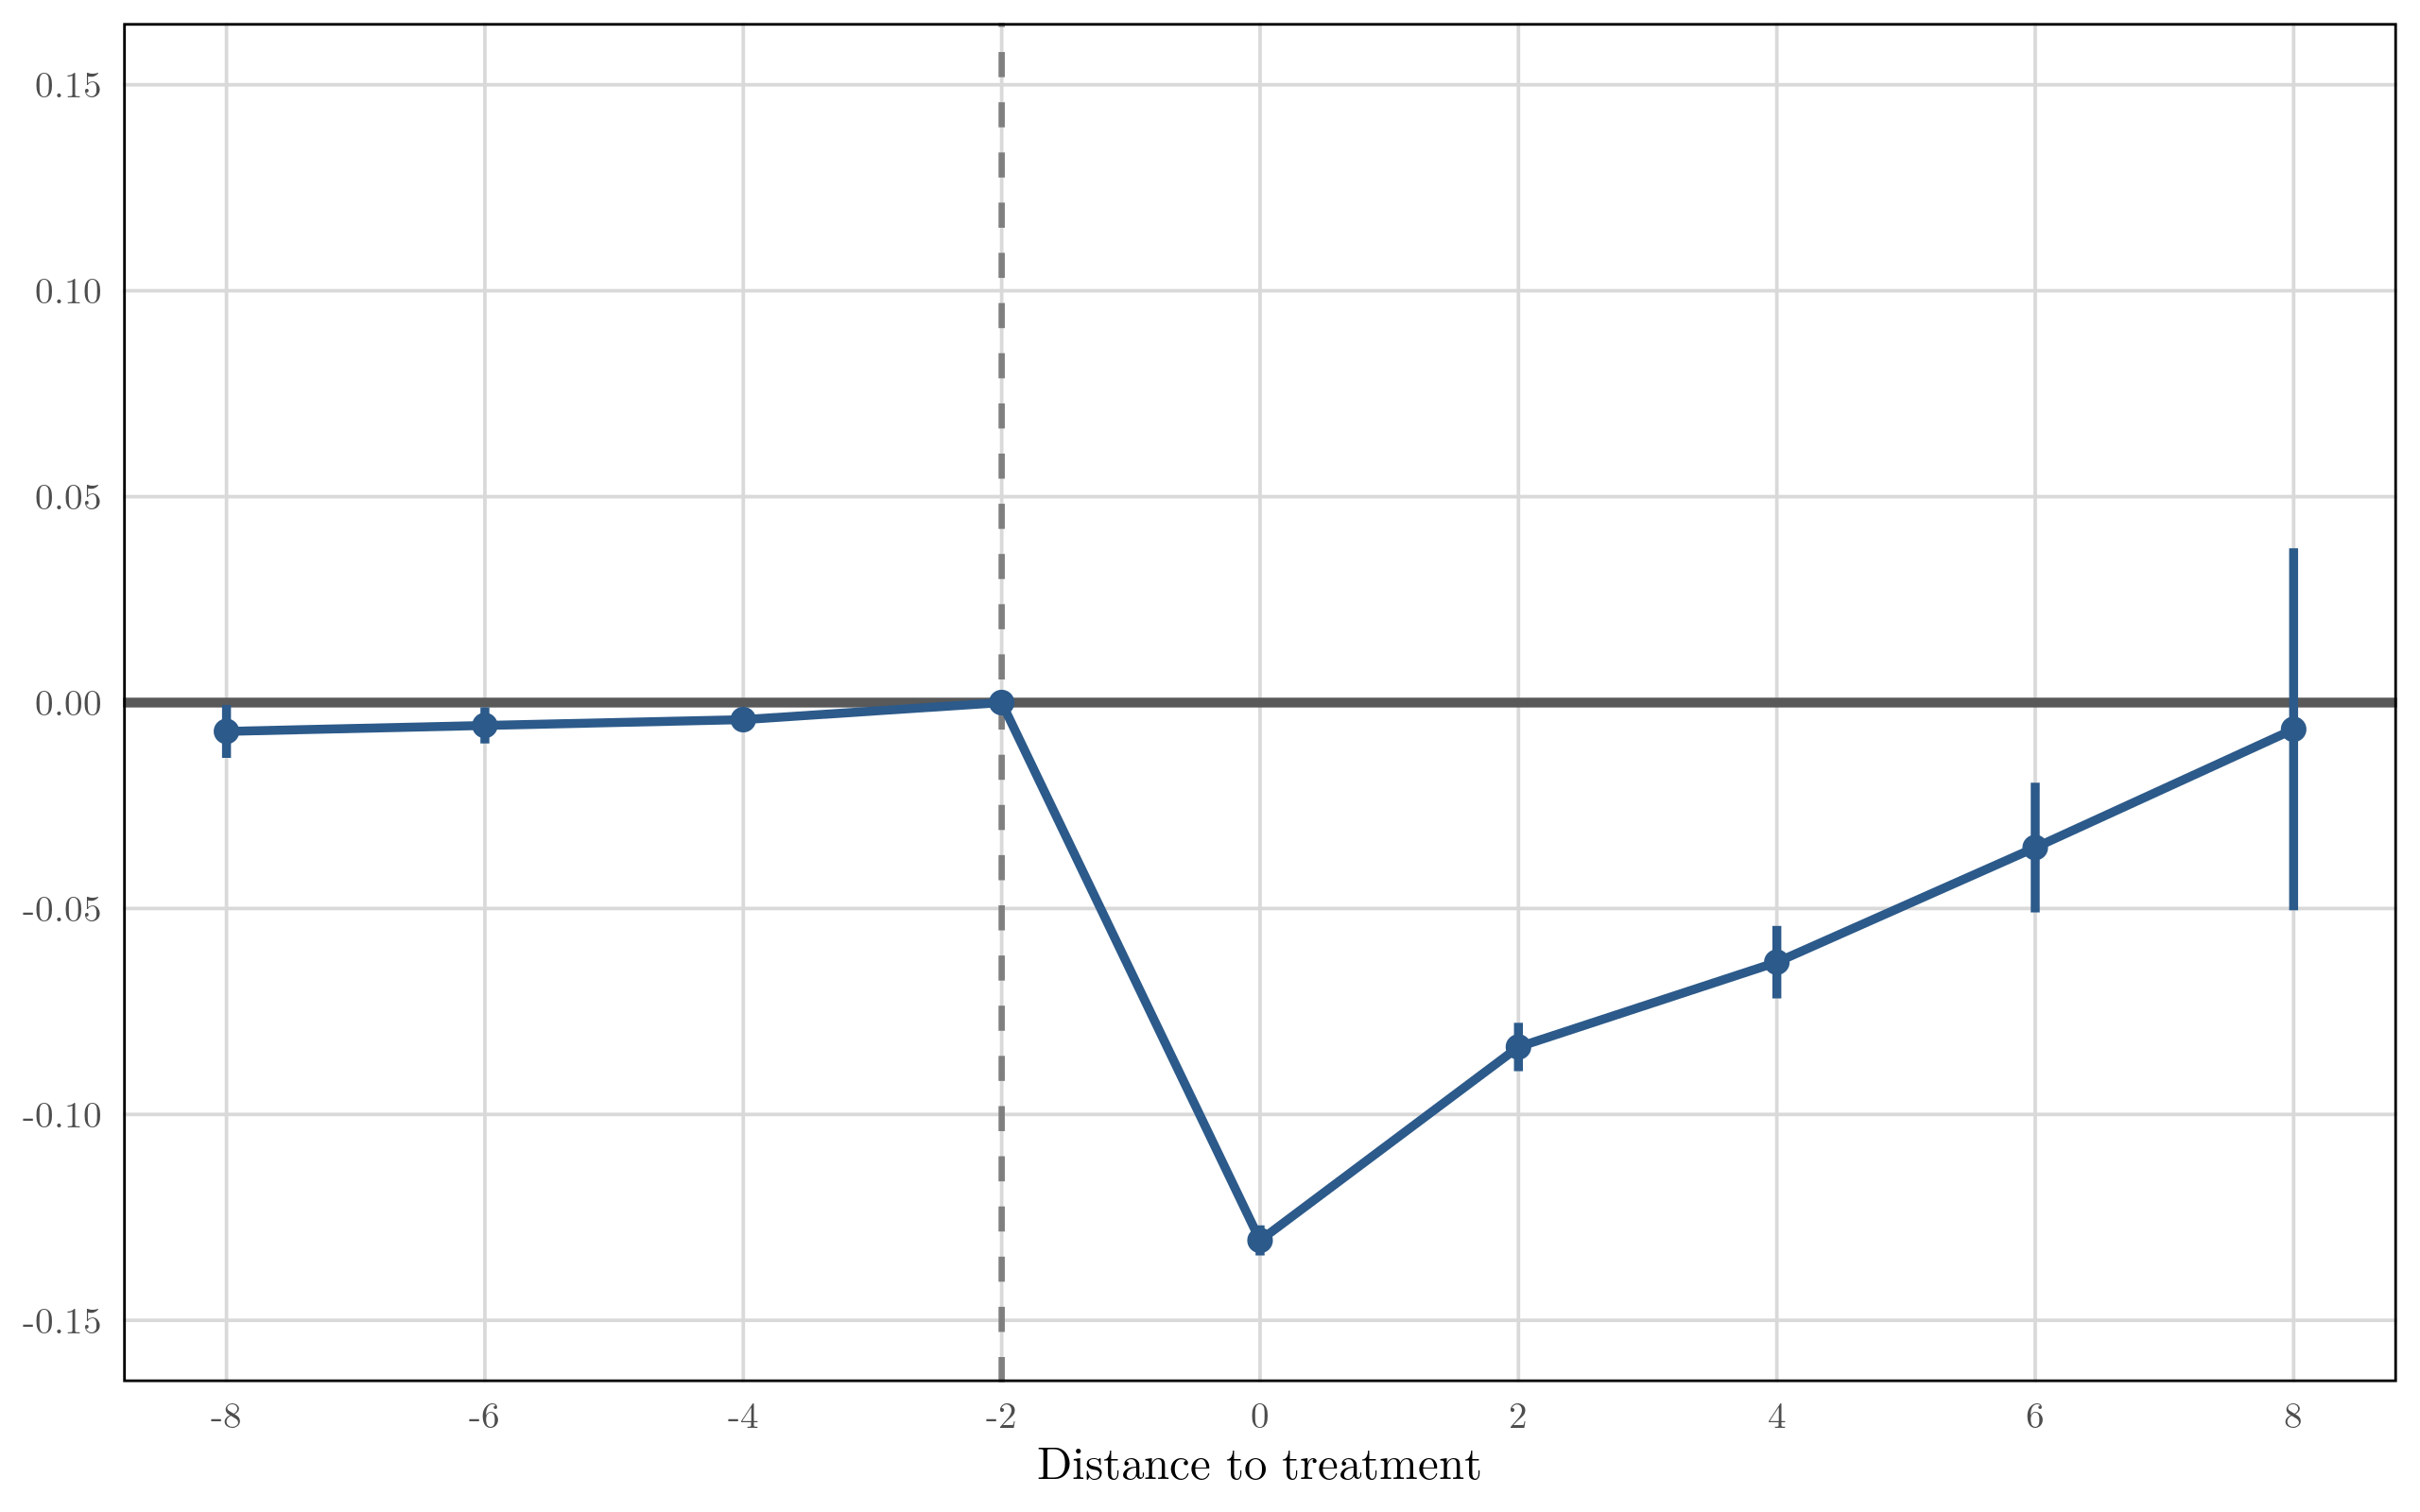
\includegraphics[width=\textwidth]{../resources/regressions/decomposition/num_voters_over_2006/strict_bvr/callaway_santanna/event_study_plot.png}
        \caption{Total electorate over 2006 total}
        \label{fig:appendix-decomp-event-total}
    \end{subfigure}
    \hfill
    \begin{subfigure}[b]{0.49\textwidth}
        \centering
        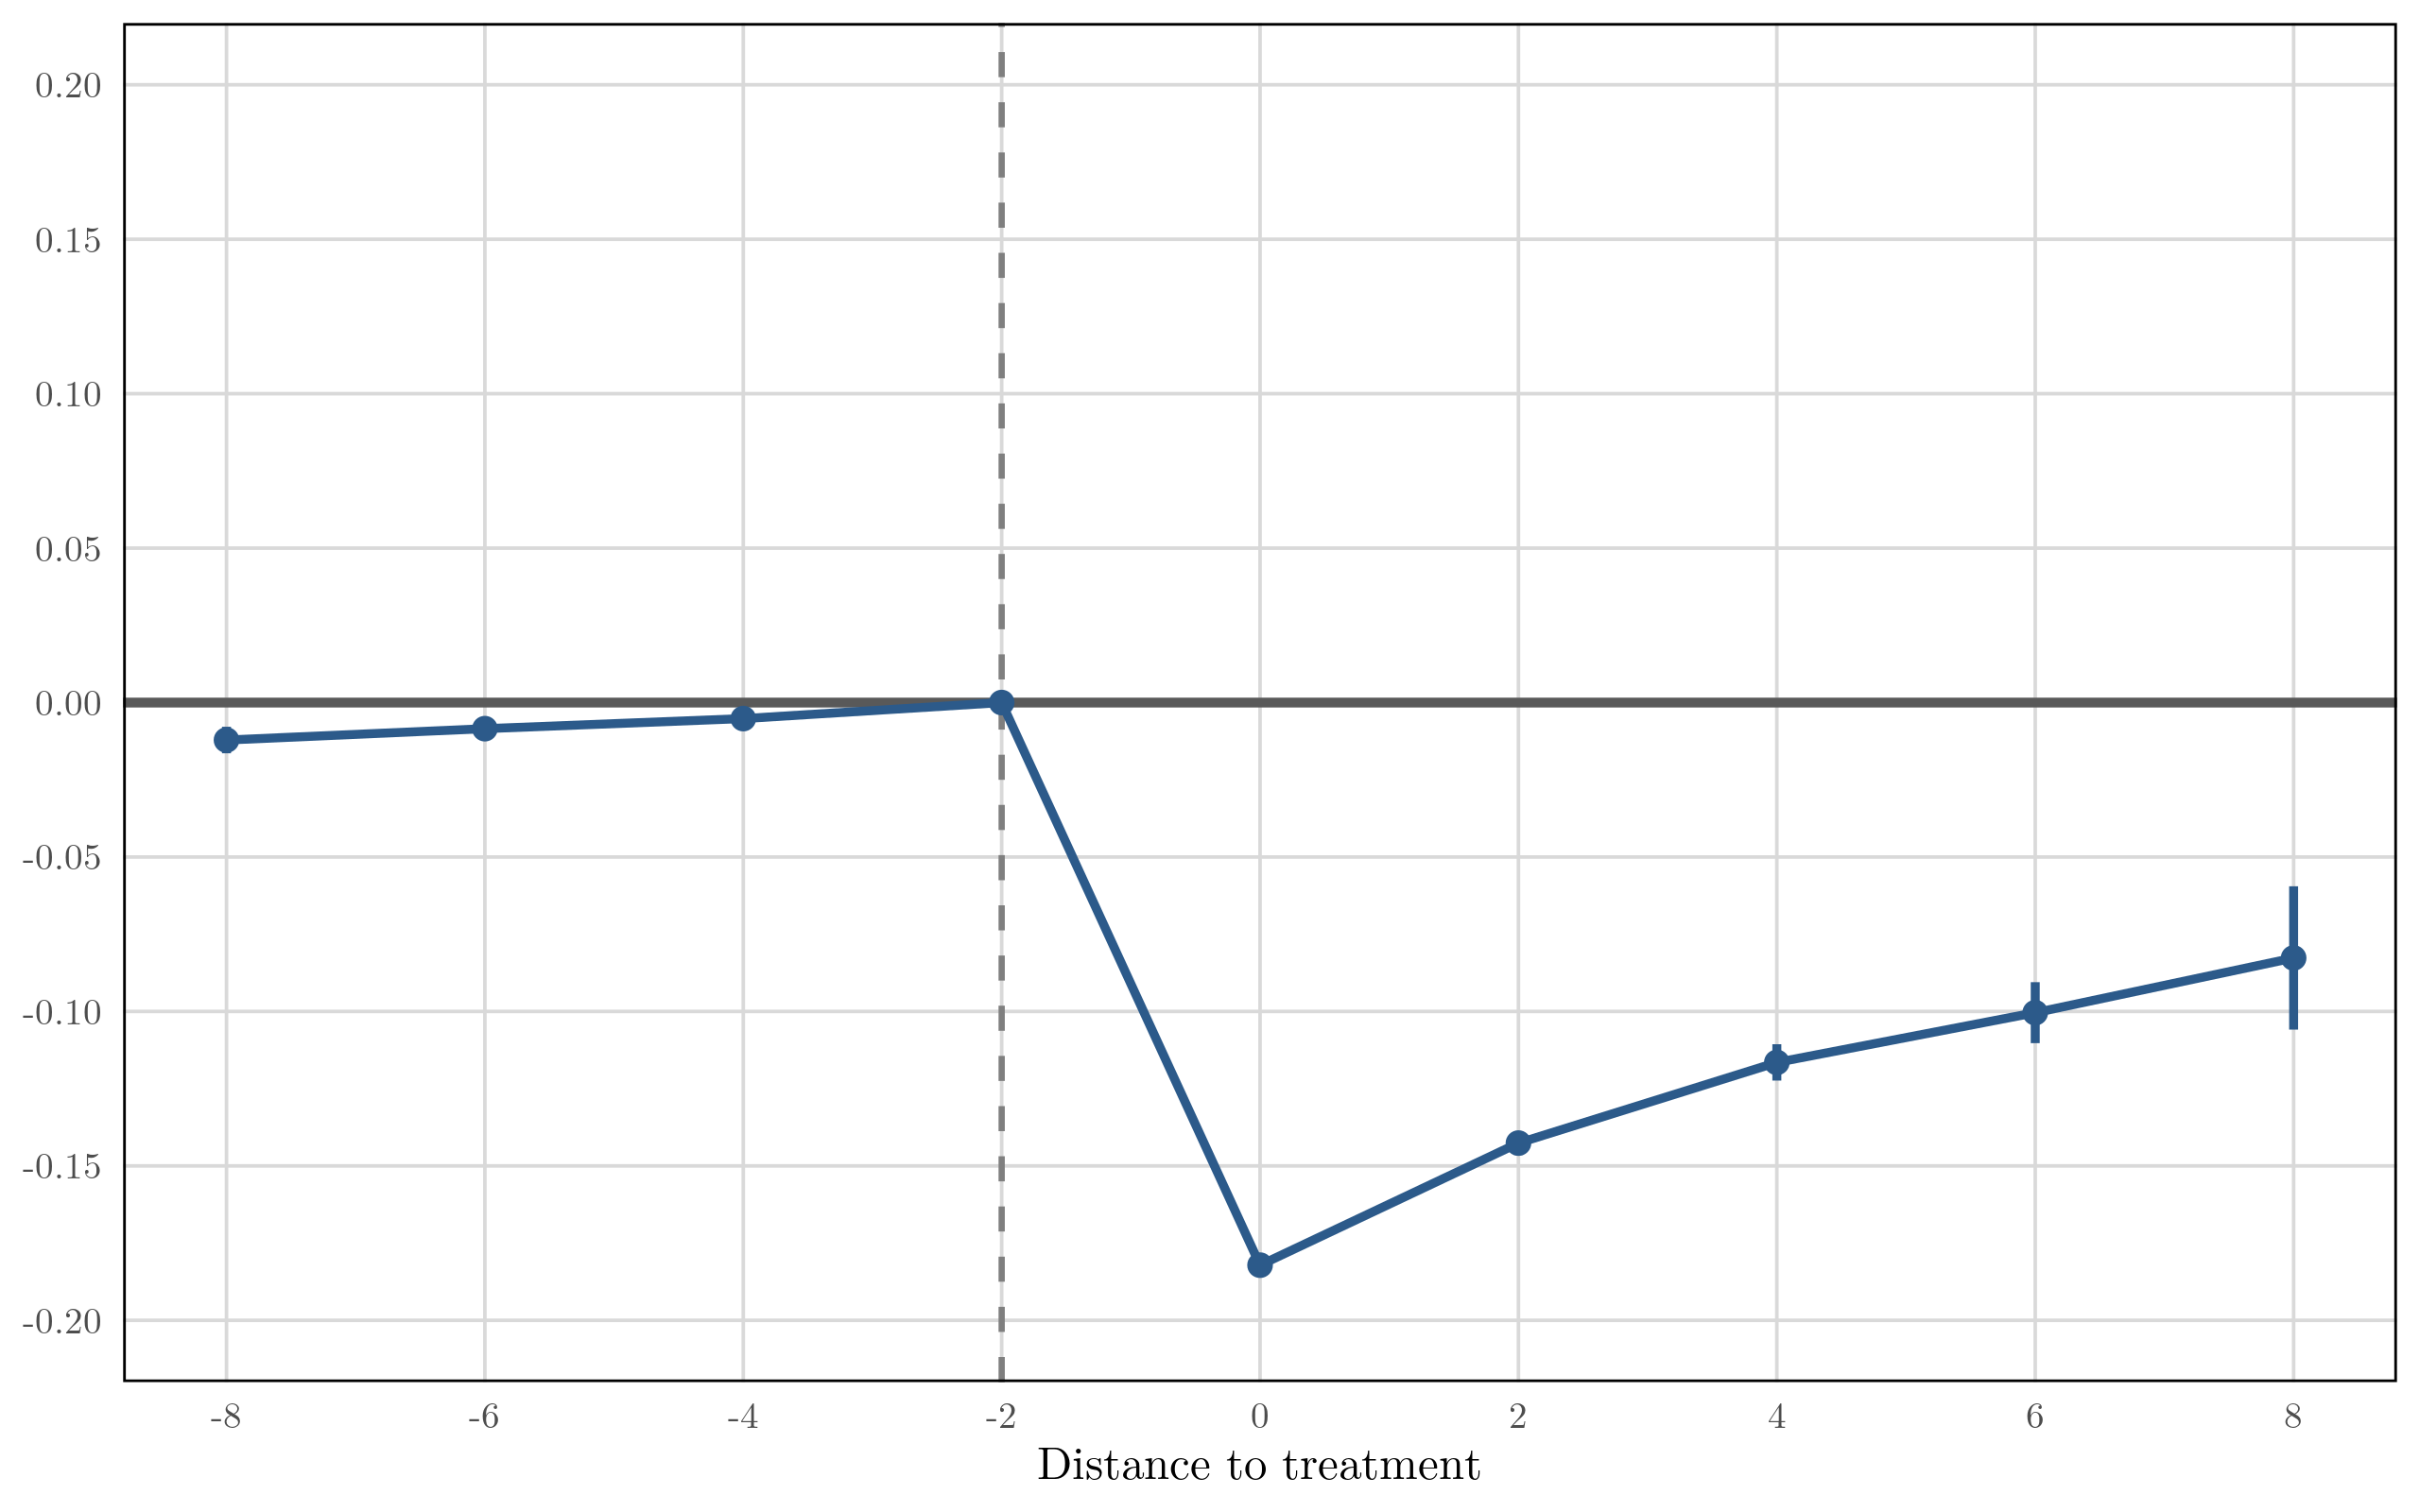
\includegraphics[width=\textwidth]{../resources/regressions/decomposition/low_ed_over_2006/strict_bvr/callaway_santanna/event_study_plot.png}
        \caption{Low education over 2006 total}
        \label{fig:appendix-decomp-event-low-ed}
    \end{subfigure}
    \par\medskip
    \begin{subfigure}[b]{0.49\textwidth}
        \centering
        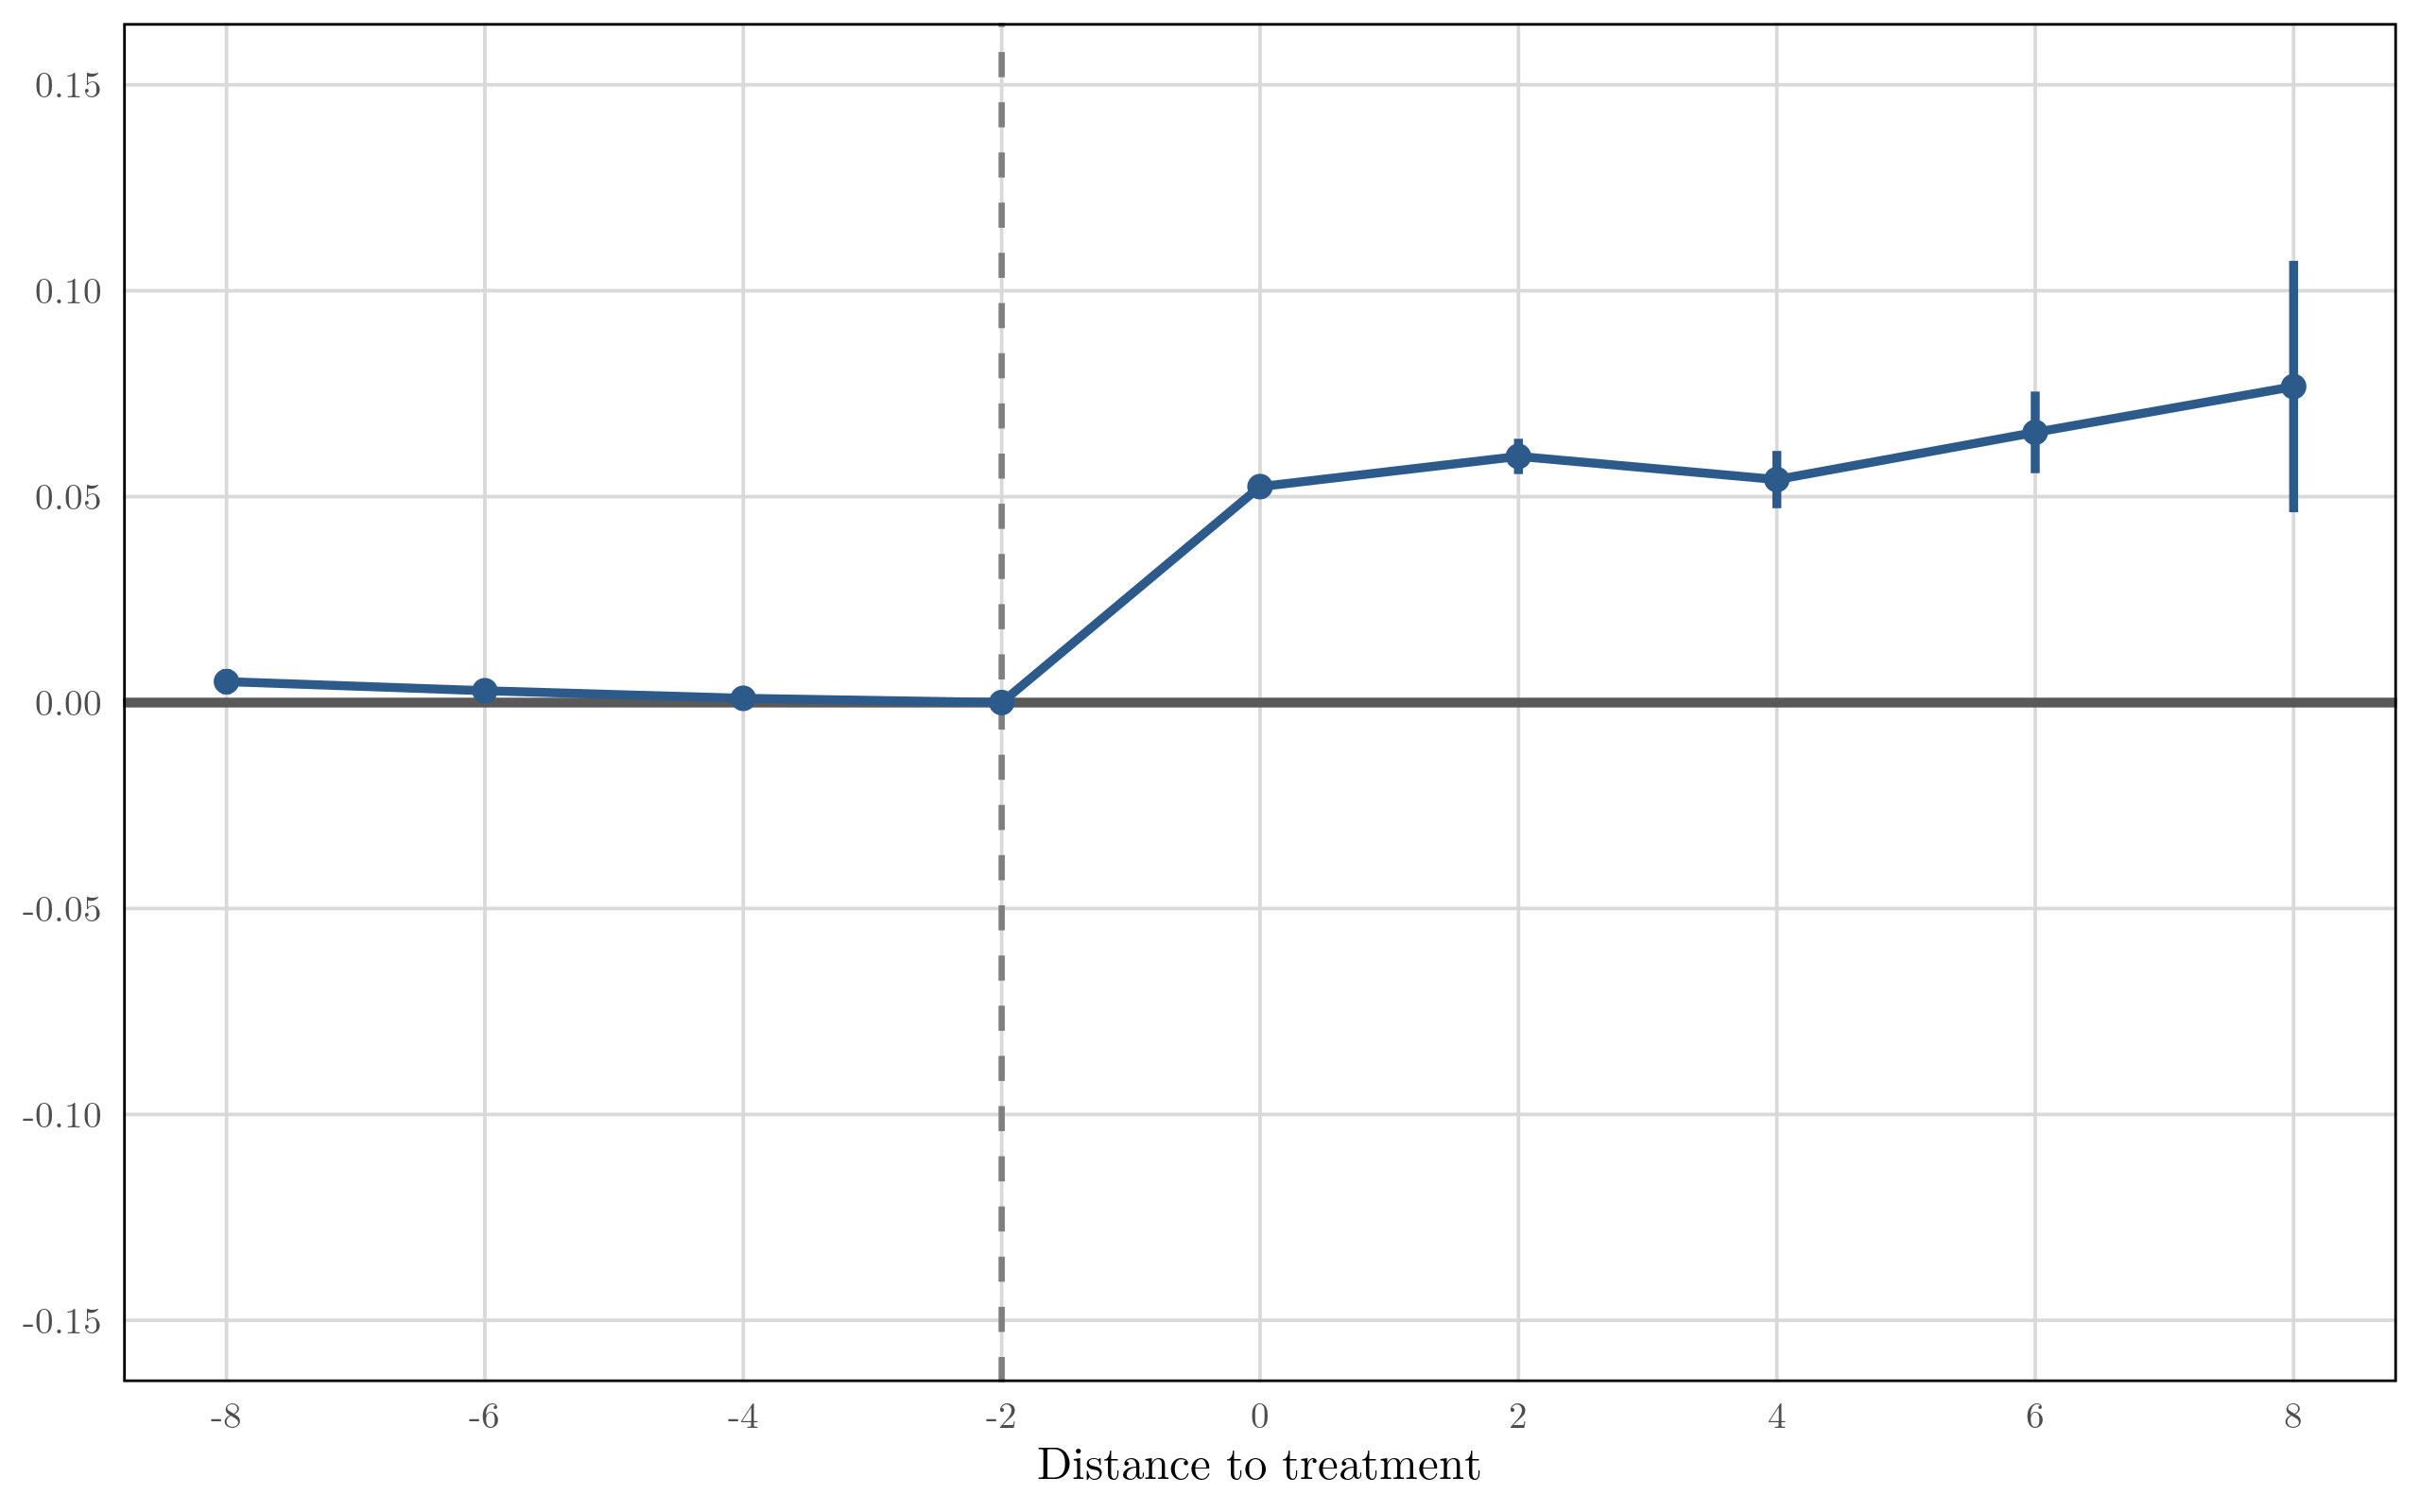
\includegraphics[width=\textwidth]{../resources/regressions/decomposition/high_ed_over_2006/strict_bvr/callaway_santanna/event_study_plot.png}
        \caption{High education over 2006 total}
        \label{fig:appendix-decomp-event-high-ed}
    \end{subfigure}
    \hfill
    \begin{subfigure}[b]{0.49\textwidth}
        \centering
        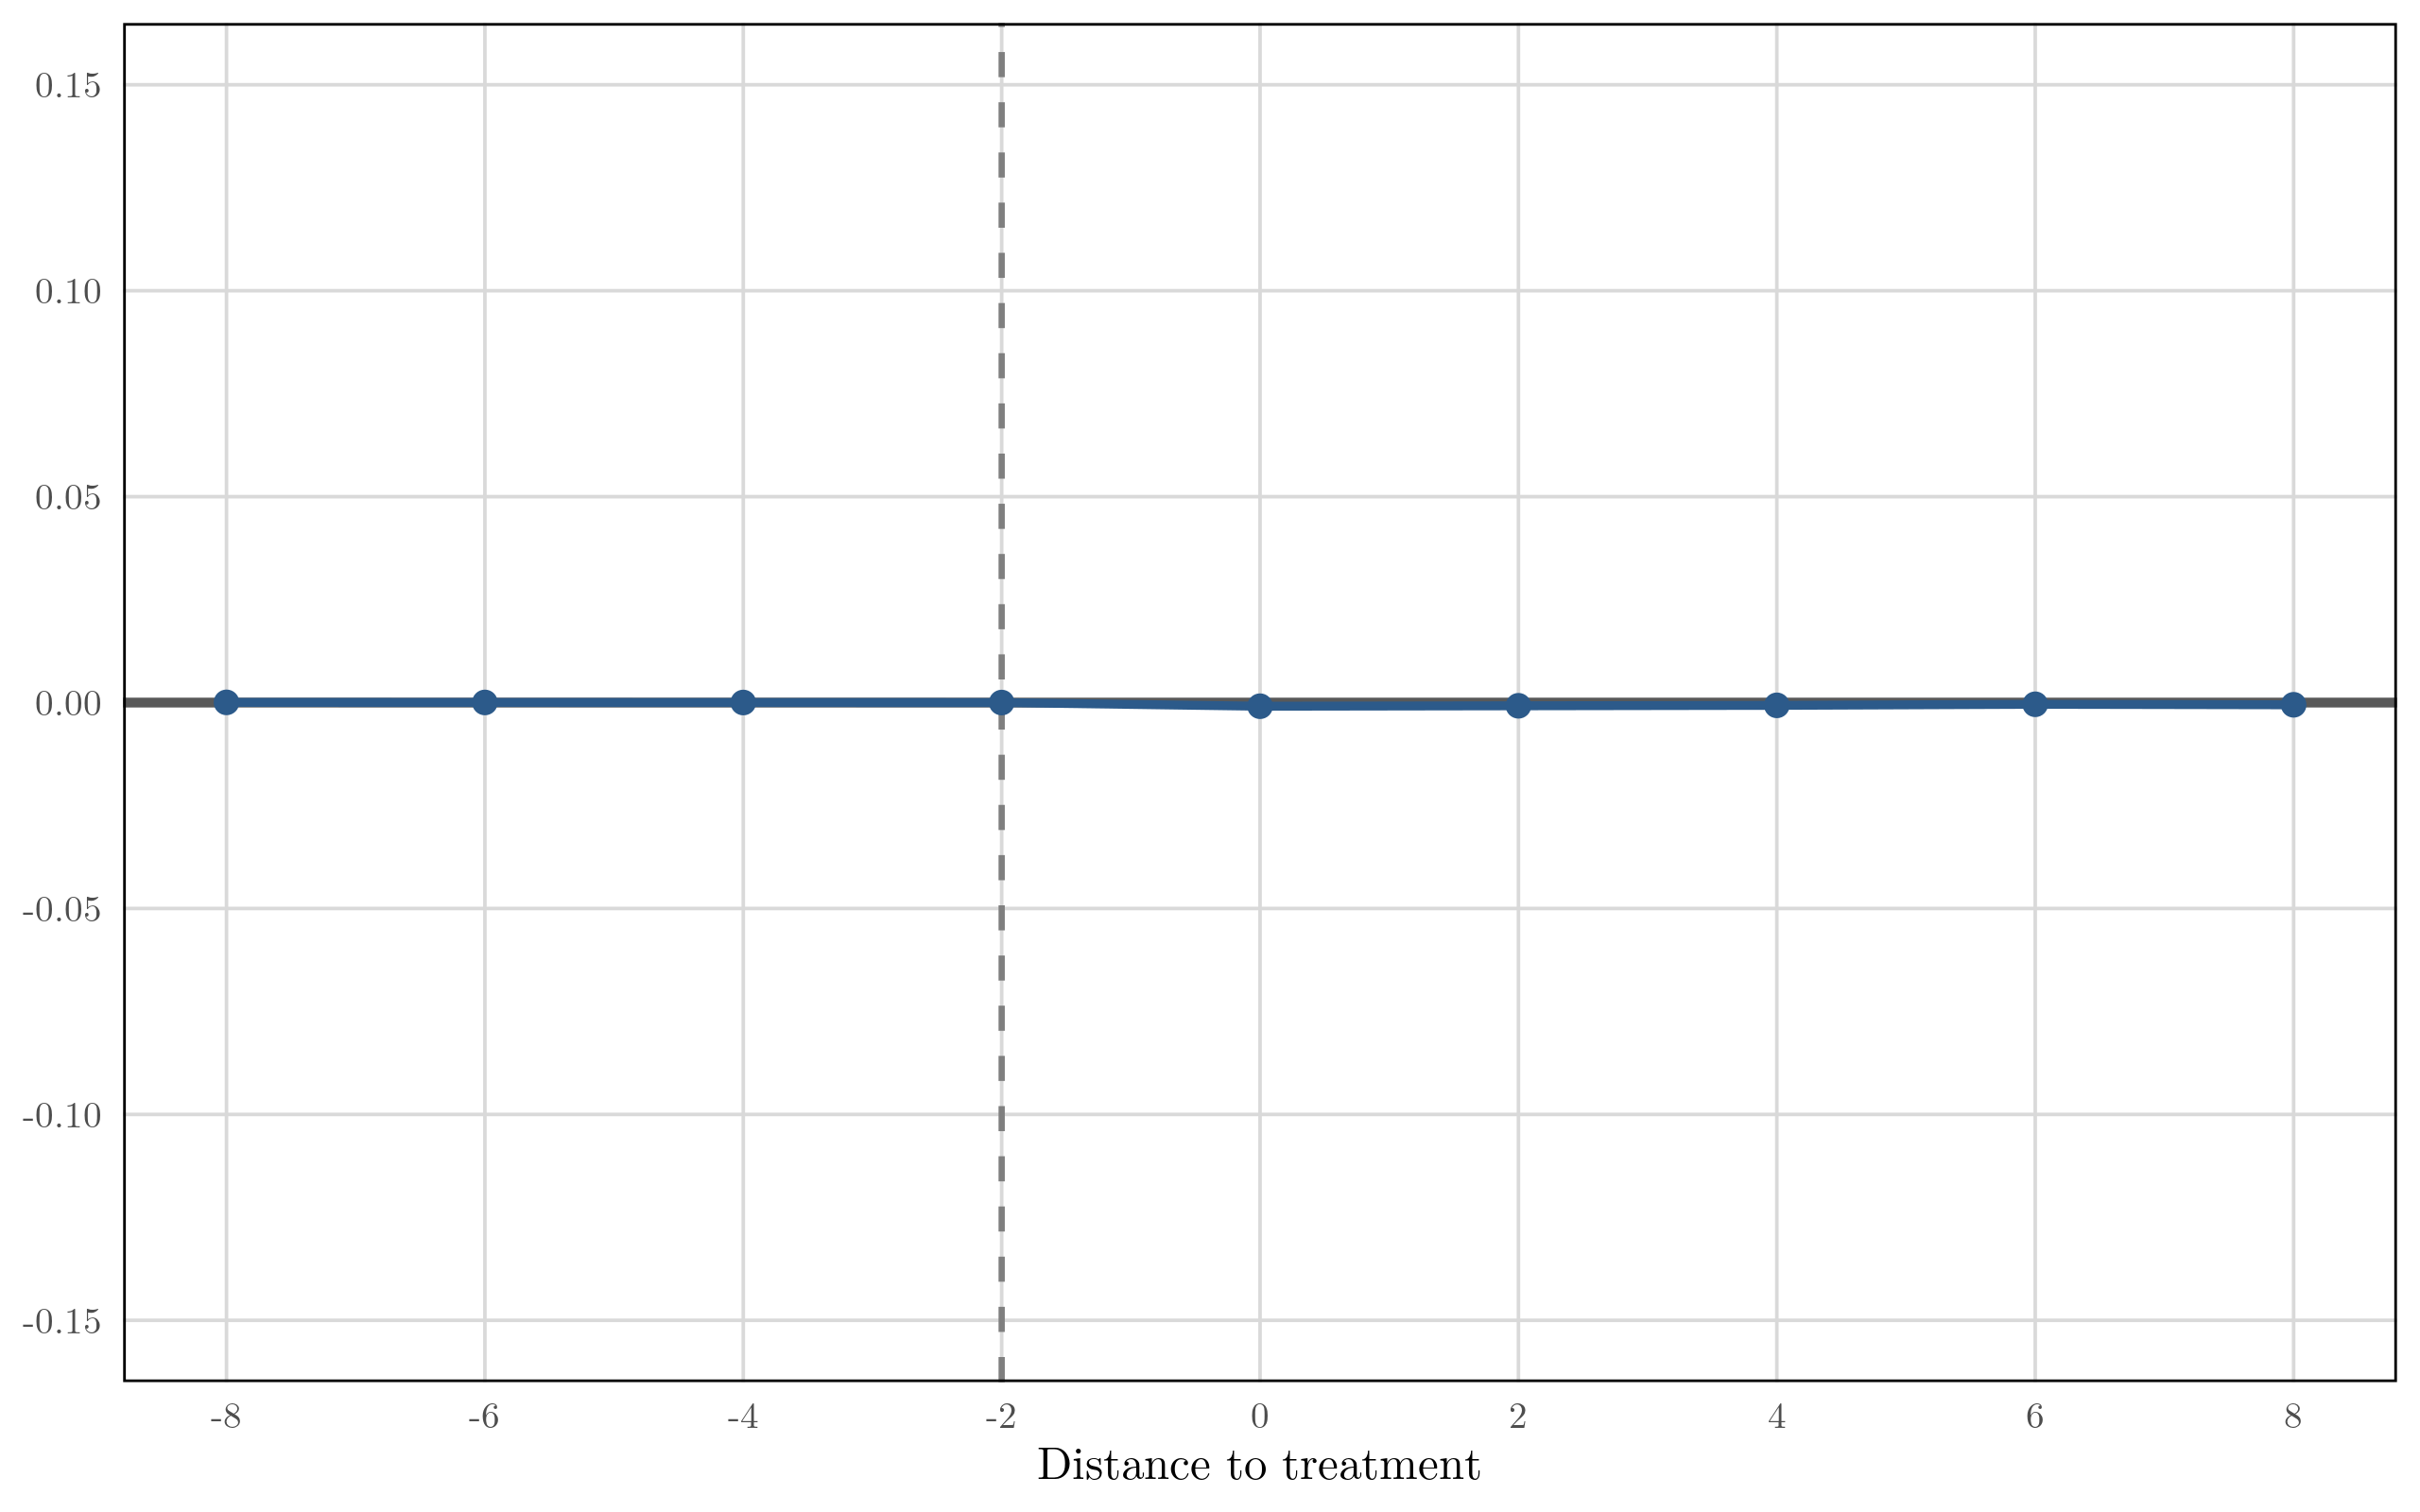
\includegraphics[width=\textwidth]{../resources/regressions/decomposition/unknown_ed_over_2006/strict_bvr/callaway_santanna/event_study_plot.png}
        \caption{Unknown education over 2006 total}
        \label{fig:appendix-decomp-event-unknown-ed}
    \end{subfigure}
    \vspace{0.75em}
    \begin{minipage}{\textwidth}
        {\footnotesize \textbf{Note:} Each panel plots BJS imputation event-study estimates \citep{Borusyak2024RevisitiEventStudy} using strict BVR municipalities as the treated sample and never-treated municipalities as the control group. Panel (a) uses total registered voters divided by the municipality's 2006 registered voters. Panels (b)--(d) use the corresponding low-education, high-education, and unknown-education counts divided by the municipality's 2006 total registered voters. Event time $-2$ is the reference period and is shown at zero. Error bars report 95\% confidence intervals with standard errors clustered by municipality. The component outcomes add to the total-electorate outcome by construction in the underlying data. \par}
    \end{minipage}
\end{figure}
